\section{Use Case Demonstration}

An example experiment was generated as a proof of concept to demonstrate a potential workflow for testing the effect of various independent variables on SfM accuracy.  


A 100m x 100m DSM was manually generated in Blender using N vertices and N unique triangular planes to represent a hilly surface.  The specular response of the surface was defined as perfectly lambertian, and the color of the surface was generated from two image textures.  The first image texture is a XX Mp seamless grass image, that was taken from a UAV at XXX.  This texture is repeated 5 times in both the X and Y dimensions, for a texel ground spacing of XX cm.  The second texture is a XMp image taken from a UAV from at xxx.  This texure is not repeated, and therefore has a texel ground spacing of XX cm.  These images are mosaiced together using an intensity value of X for the repeating grass texture, and an intensity value of Y for the overview image.  Both textures are interpolated in the renderer to avoid crisp edges or corners in between texels.  A large 5m x 5m cube is placed in the center of the scene to observe the inability of SfM to generate crisp corners.  The cube is textured using a XMp image of asphalt that was taken by a DSLR.  The texel ground spacing is XX cm.  Eleven 0.5m x 0.5m Black and White Checkered, lambertian GCPs are distributed in the scene to simulate being laid on the simulated hilly surface in an adhoc manner.  To illuminate the scene, the sun is placed at a nadir angle for the first image, and its angle is linearly interpolated about the x axis so that the final image is rendered with a 30 degree solar incident angle.  The ray tracing algorithm is set up so that shadows are cast by objects within the scene.  An ambient light source for the environment is set to be 10\% the value of the solar illumination, to prevent shadowed areas from rendering completely black.  

A trajectory is generated in Matlab to simulate the motion of a small action camera on a UAS at an altitude of 25 meters flying a grid pattern across the scene with X sidelap and X overlap.  To avoid imaging the edge of the simulated hilly topography, the outermost 10 meters of the scene are not considered in the simulated flight planning.  The camera pose is nadir, but with a $\pm 5 \degree$ random offset in roll, pitch, and yaw angles of the uas.  The Blender Internal Render was used to render 100 images, which took approximately X minutes on a XX computer.  To simulate more nonidealized imagery, the raw images were postprocessed to add gaussian blur, gaussian noise, salt and pepper noise, and nonlinear distortion governed by the brown distortion model using a Matlab script.

The postprocessed imagery was loaded into Agisoft Photoscan (version XX), and processed with settings shown in Table X.  Notice that the GCP positions, camera positions, and camera interior orientation are input with no uncertainty, since the scene has been simulated.  Additionally, the pixel coordinates of the GCPs, which are traditionally clicked by the user by varying degrees of accuracy are calculated using photogrammetric equations and input into the program.  The accuracy of the control points as reported by Photoscan are shown in Table X.  Note that as a result of the unrealistic accuracy and of the data input into the program, the errors are reported in millimeters.  This is not realistic to expect from a real world scenario, but provides an example best case scenario for what to expect from SfM. The result of the processing is an orthophoto, with 1cm resolution, a sparse pointcloud with N points, and a dense pointcloud with N points.  These data are then compared to the groundtruth data, which in this case is the model and a simulated orthophoto from Blender.  

\subsection{Experiment Design}
A 200 meter square surface was manually generated to simulate a topography with rolling hills using a 1 meter grid.  A large 3 meter cube was placed in the center of the scene to test surface reconstruction accuracy on regions with sharp corners and edges.  Ten 1m x 1m x 0.05m square Ground Control Points (GCPs) are distributed evenly throughout the scene 0.25 meters above the ground surface.  The material of all the objects in the scene are as perfect lambertian surfaces.  The topographic surface was textured using a combination of two textures.  The first texture is a 7200x7200 pixel aerial image \todo{cite NZ} for an effective texel footprint of 2.78cm square.  The second texture is a 3456x3456 pixel image of grass was tiled ten times in both the x and the y dimension for an effective texel footprint of 0.58cm square.  The image of grass was taken with a DSLR and manually edited to create a seamless texture for tiling.  The aerial image and grass texture were merged together by setting their alpha values to 1 and 0.15 respectively.  The cube was textured using a 3456x3456 pixel seamless image of rocks that was derived from a DSLR image taken by the authors.  This resulted in an effective texel footprint of 0.35cm square.  Each of the textures is set so that the coloring on the scene is interpolated between texels so that there are no abnormal effects on the edge of pixels.  An aerial image and oblique image of the scene are shown in \figref{fig:scene}. \todo{make this figure better. break into 2 figures. one shows layout of cameras and GCPs, one shows close up of gcp and box}

The scene was illuminated using a "Sun" lamp, which begins at directed at nadir and is linearly interpolated to a 30 degree rotation about the x axis for the final image. The sun has a constant intensity of 1, and emits white light with values of 1 for the R,G, and B.  To improve lighting in shadowed regions, an ambient light source was added with an intensity value of 0.25 and values of 1 for R,G, and B.  

\begin{figure}[H]
	\centering
	\includegraphics[height = 1.5in]{../fig/scenesummary}

	\caption{The scene was generated in Blender to represent a hilly topography(left) with 10 Ground Control Points (center) distributed throughout the scene and a 3m cube placed in the center(right).}
	\label{fig:scene}
\end{figure}

A camera is created in Blender with parameters meant to emulate a Sony A5000 with a 16mm lens and 5456x3632 pixel sensor.  A flight path is generated to create a Ground Sampling Distance (GSD) of 1.00cm and an overlap and sidelap of 75\% each.  In order to reduce imaging the edge of the topographic surface, the inner 100 meters of the topography are selected as the Area of Interest.  Using these constraints, a trajectory consisting of 77 exterior orientations distributed across 7 flight lines is generated with nadir looking imagery.  In order to generate imagery that is more representative of a real world scenario with an unstable UAS, 1 sigma gaussian noise in meters is added to the camera translation in each of the three dimensions and 2 sigma gaussian noise in degrees is added to the camera rotation about each of the three axes.  Imagery is then rendered using Blender Internal Renderer with the default 8-sample antialiasing enabled.

The imagery that is output from Blender is postprocessed in Matlab to simulate nonlinear brown distortion \todo{cite brown distortion}, vignetting, salt/pepper noise, gaussian noise, and gaussian blur.  In order to adequately apply fisheye distortion and gaussian blur, the imagery was rendered at a larger resolution that the sensor and then cropped.  The constants used in this postprocessing are shown in \tabref{tab:postproc}  
\todo{need to add equations for brown distortion, vignetting, add distortion eqn units, etc... this could get cumbersome...}

% Table generated by Excel2LaTeX from sheet 'Parameter Distributions'
\begin{table}[htbp]
  \centering
  \caption{.}
    \begin{tabular}{lrr}
    	\toprule
    Parameter & Value & units \\
    \midrule
    Distortion $k_1$ & -4    & f \\
    Distortion $k_2$ & -4    & f \\
    Distortion $k_3$ & -4    & f \\
    Distortion $k_4$ & -4    & f \\
    Distortion $p_1$ & -4    & f \\
    Distortion $p_2$ & -4    & f \\
	Vignetting $v_1$ & 10    & DN \\	
    Vignetting $v_2$ & 0.2   & DN \\
    Vignetting $v_3$ & 0     & DN \\
    Salt Noise Probability & 0.01 & \% \\
    Pepper Noise Probability & 0.01 & \% \\
    Gaussian Noise Mean & 0 & DN \\
    Gaussian Noise Variance & 0.02 & DN \\
    Gaussian Blur Sigma & 1 & \\
    \bottomrule
    \end{tabular}%
  \label{tab:postproc}%
\end{table}%

\subsection{Processing Methodology}
The resultant imagery was processed using the commercial software Agisoft Photoscan Pro using the settings shown in \todo{cite table}.  The dataset was processed by inputting the position of the cameras, the position of the GCPs, the associated pixel coordinates of each GCP, and the camera calibration file with no uncertainty or error added.  A nonlinear adjustment is performed using the "optimize" button, and the reported total RMS for the GCPs is 0.38mm.  This represents an idealized scenario which is unattainable in a real world scenario as traditionally there will be error in the GCP surveyed markers, the UAS position, the user clicking of pixel coordinates for GCPs, and in the calculation of the camera calibration.  

A dense reconstruction is performed using the "aggressive" filtering and each of the quality settings available in Photoscan.  The quality settings downsample the imagery for faster processing, and ultrahigh becomes quickly unattainable to users without purpose built CPUs with large amount of RAM. \todo{better describe quality and cite photoscan manual}. The processing time and number of points for each pointcloud is shown in Table X.  The computer used is a Windows 7 Desktop PC with a Intel Xeon CPU E5-1603 @ 2.80GHz, GeForce GTX 980 Graphics card (4Gb), and 32Gb of RAM.

% Table generated by Excel2LaTeX from sheet 'Sheet7'
\begin{table}[htbp]
  \centering
  \caption{Add caption}
    \begin{tabular}{lcrrr}
   	\toprule
    Pointcloud Name & Time (Hours:Minutes) & Number of Points & RMSE Mean (m) & RMSE std (m)\\
    \midrule
    sparse          & 00:36 & 22,214       & -0.0001  & 0.0028 \\
    dense lowest    & 00:03 & 716,331      & -0.0066  & 0.0323 \\
    dense low       & 00:09 & 2,886,971    & -0.0020  & 0.0154 \\
    dense medium    & 00:30 & 11,587,504   & -0.0005  & 0.0077 \\
    dense high      & 02:19 & 46,465,218   & -0.0002  & 0.0044 \\
    dense ultrahigh & 11:54 & 186,313,448 & -0.0002  & 0.0026 \\
    \bottomrule
    \end{tabular}%
  \label{tab:pctime}%
\end{table}%


Each of the dense pointclouds is brough into the CloudCompare \todo{cite} and compared to the groundtruth blender mesh using the "point to plane" tool.  This tool calculates this signed distance of every point in the pointcloud to the nearest surface on the mesh, using the surface normal to determine the sign.  This distance is referred to as the error.  Each pointcloud was then analyzed in Matlab to determine how the dense reconstruction quality setting effects the reconstruction error.

\subsection{Results}

The error was first visualized spatially for each reconstruction by gridding the pointcloud elevation and error using a nearest neighbor gridding technique.  The number of points and standard deviation of points in each grid cell are also visualized.  The results for the medium quality dense reconstruction are shown in \figref{fig:spatial}.  These plots are useful to begin to explore any spatial correlations in the data.  One observation is that in the standard deviation of error plot there is higher uncertainty at the edges of the pointcloud beyond the AOI.  This is due to the poor viewing geometry at the edges of the scene.  \todo{need to make this better}

\begin{figure}[H]
	\centering
	\includegraphics[height = 5in]{../fig/spatialmedium}

	\caption{The elevation, error, number of points, and standard deviation of error are gridded to 0.5 meter grid cells using a nearest neighbor gridding algorithm and visualized.}
	\label{fig:spatial}
\end{figure}

To qualitatively observe the effect of different quality dense reconstructions, a plot showing a 0.5 meter wide section of the center of the box is shown in \figref{fig:boxplot}. \todo{add caption} 

\begin{figure}[H]
	\centering
	\includegraphics[height = 3in]{../fig/boxprofile}

	\caption{add caption.}
	\label{fig:boxplot}
\end{figure}

A more quantitative, statistical assessment is performed by calculating the distribution of error for each pointcloud, as shown in \figref{fig:hist}. \todo{add caption}

\begin{figure}[H]
	\centering
	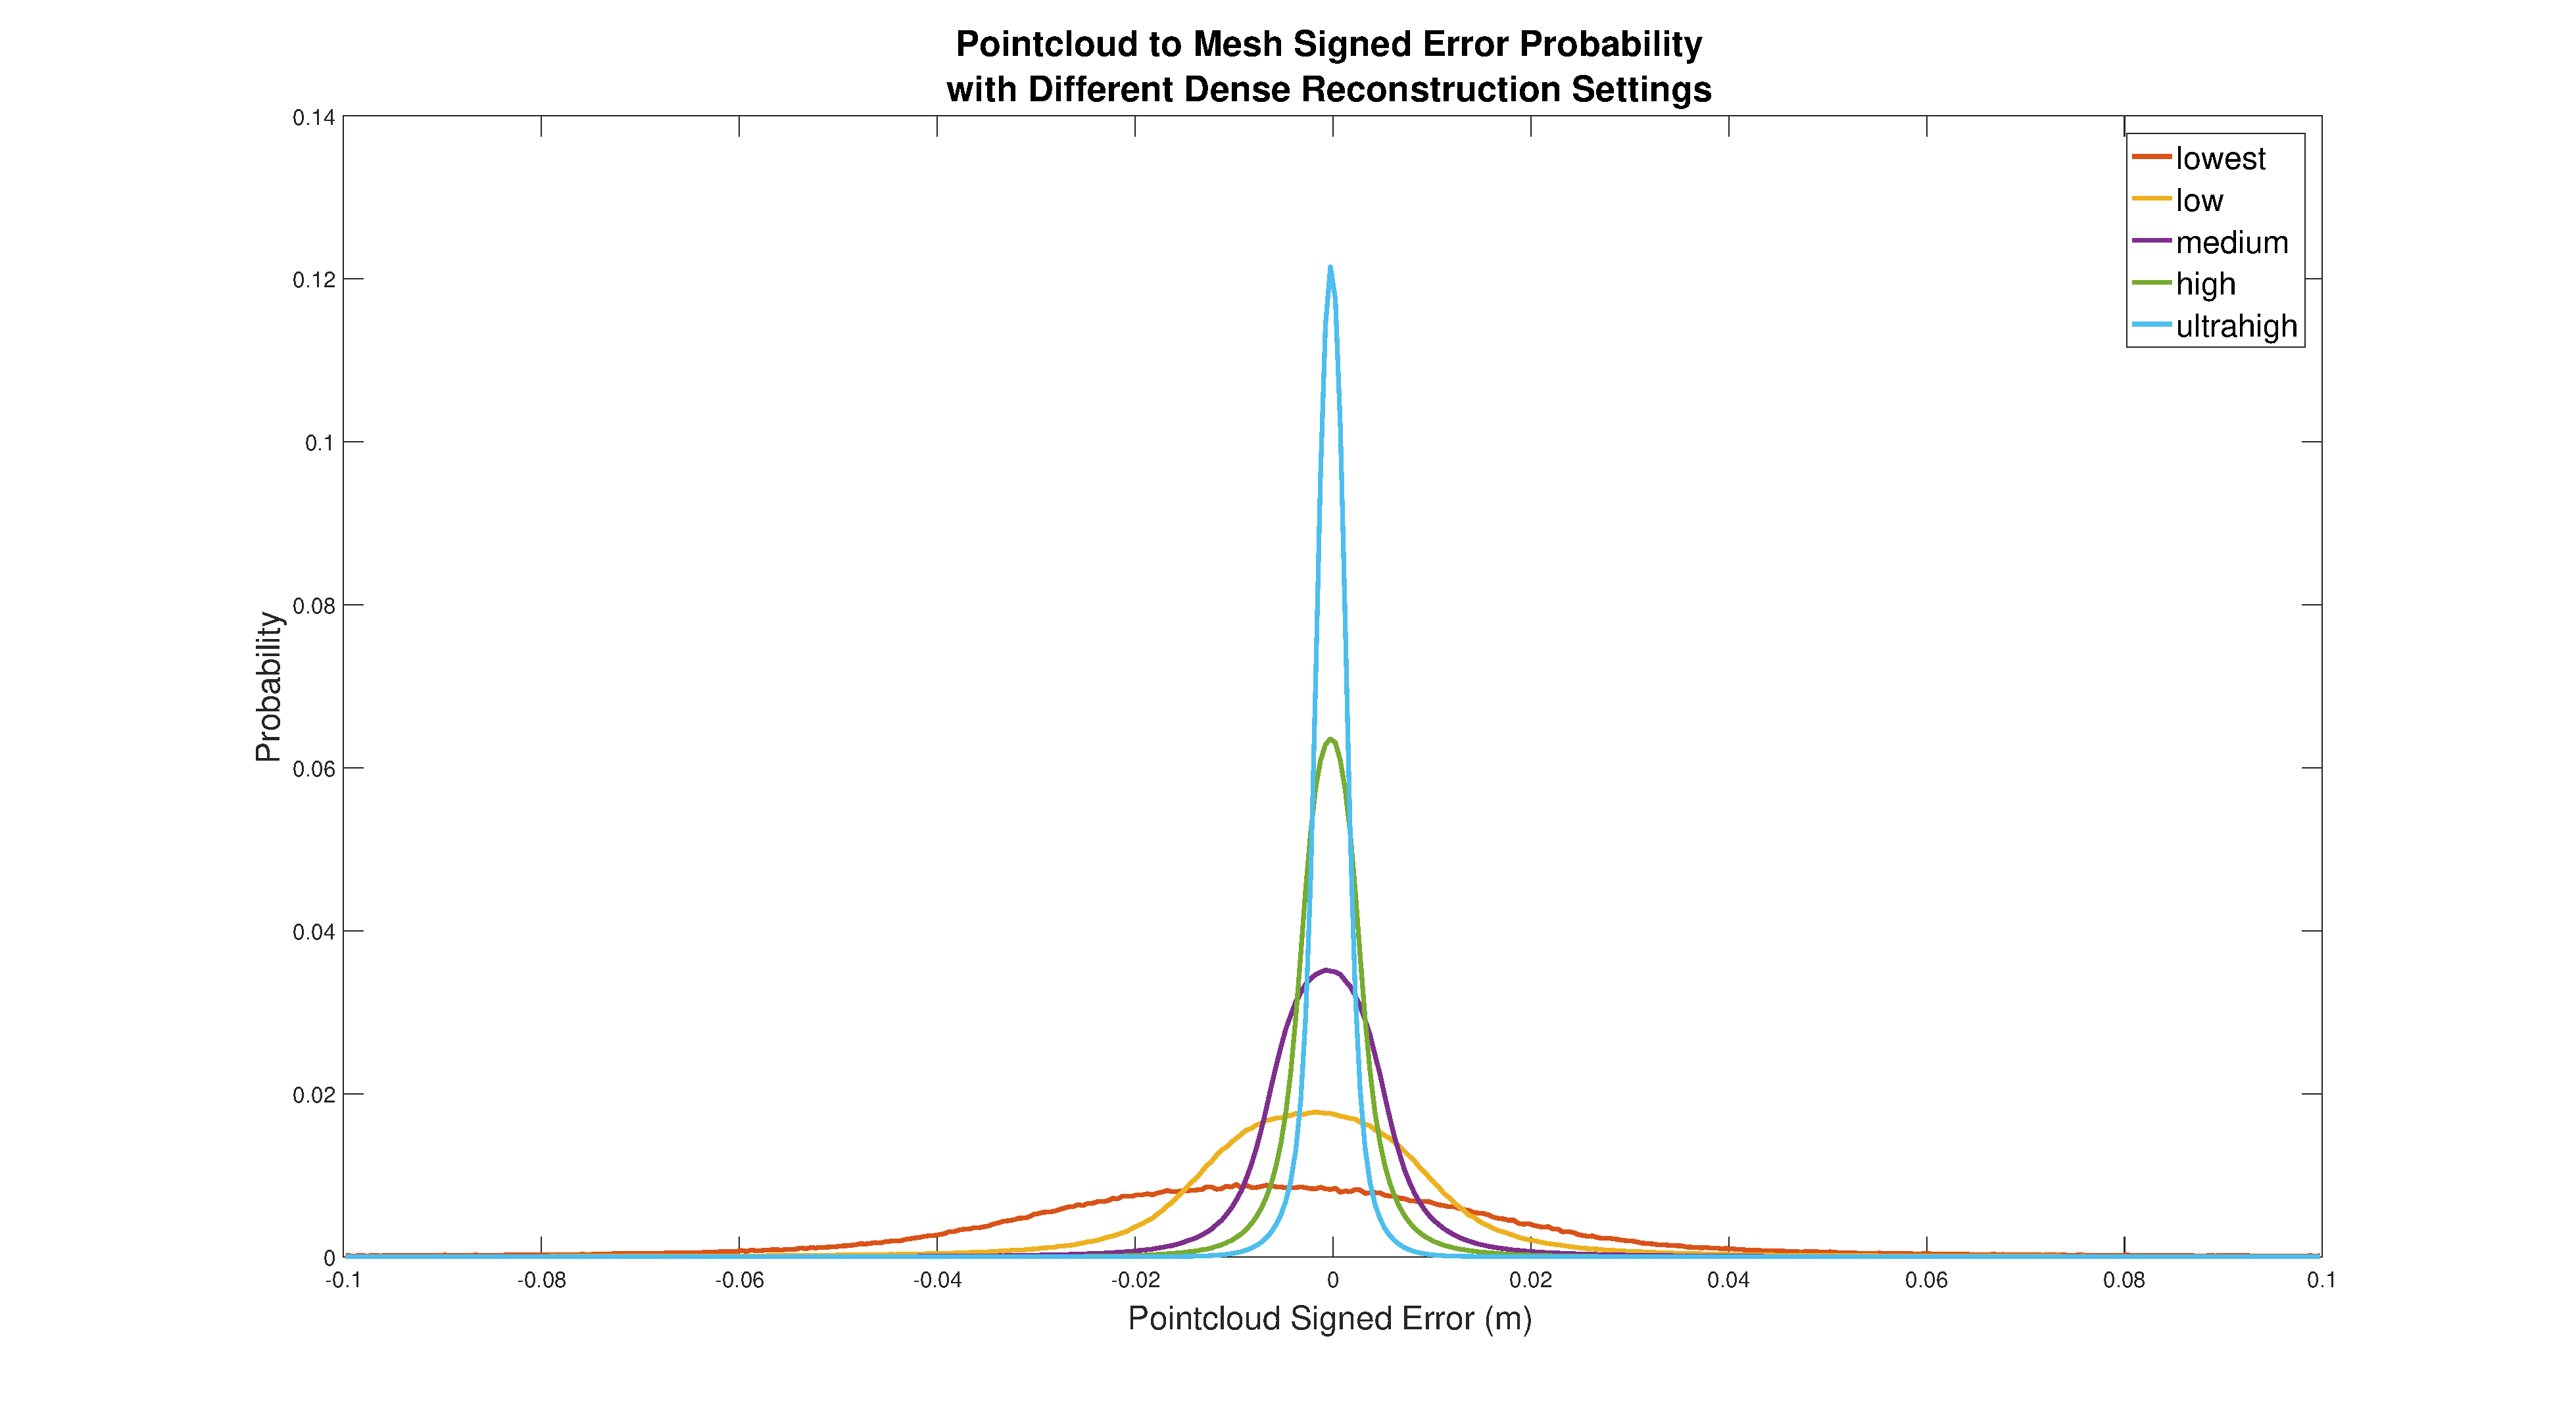
\includegraphics[height = 3in]{../fig/histerror}

	\caption{add caption.}
	\label{fig:hist}
\end{figure}



%Sourced from Orthophoto AT25. Crown Copyright Reserved. http://www.linz.govt.nz/topography/aerial-images/nztm-geo/bj36
	
